\documentclass[12pt,a4paper]{article}

% ===== Packages =====
\usepackage[utf8]{inputenc}
\usepackage[T1]{fontenc}
\usepackage{geometry}
\usepackage{graphicx}
\usepackage{booktabs}
\usepackage{array}
\usepackage{longtable}
\usepackage{xcolor}
\usepackage{hyperref}
\usepackage{listings}
\usepackage{caption}
\usepackage{subcaption}
\usepackage{tikz}
\usepackage{float}
\usepackage{fancyhdr}
\usepackage{titlesec}
\usepackage{enumitem}
\usepackage{tcolorbox}

% ===== Page Geometry =====
\geometry{margin=1in}

% ===== Colors =====
\definecolor{greengold}{RGB}{34,120,60}
\definecolor{darkgreen}{RGB}{0,80,40}
\definecolor{codebg}{RGB}{245,245,245}
\definecolor{codeframe}{RGB}{200,200,200}

% ===== Hyperref Setup =====
\hypersetup{
    colorlinks=true,
    linkcolor=darkgreen,
    urlcolor=greengold,
    citecolor=darkgreen
}

% ===== Code Listing Style =====
\lstdefinestyle{arduino}{
    backgroundcolor=\color{codebg},
    frame=single,
    rulecolor=\color{codeframe},
    basicstyle=\ttfamily\footnotesize,
    keywordstyle=\color{blue}\bfseries,
    commentstyle=\color{gray}\itshape,
    stringstyle=\color{red},
    numbers=left,
    numberstyle=\tiny\color{gray},
    numbersep=8pt,
    breaklines=true,
    showstringspaces=false,
    tabsize=2,
    language=C++,
    morekeywords={pinMode, digitalWrite, analogRead, Serial, lcd, map, constrain, millis, delay, OUTPUT, INPUT, HIGH, LOW, A0, A1}
}

% ===== Header / Footer =====
\pagestyle{fancy}
\fancyhf{}
\fancyhead[L]{\textcolor{greengold}{\textbf{GreenGold OS}}}
\fancyhead[R]{\textcolor{gray}{IoT Smart Bin -- Proteus Simulation Plan}}
\fancyfoot[C]{\thepage}
\renewcommand{\headrulewidth}{1.5pt}
\renewcommand{\headrule}{\hbox to\headwidth{\color{greengold}\leaders\hrule height \headrulewidth\hfill}}

% ===== Title Formatting =====
\titleformat{\section}{\Large\bfseries\color{darkgreen}}{\thesection}{1em}{}
\titleformat{\subsection}{\large\bfseries\color{greengold}}{\thesubsection}{1em}{}

% ===== Document =====
\begin{document}

% ===== Title Page =====
\begin{titlepage}
\centering
\vspace*{1cm}

{\Huge\bfseries\textcolor{darkgreen}{GreenGold OS}}\\[0.5cm]
{\Large\textcolor{greengold}{Smart Waste Management System}}\\[2cm]

\rule{\textwidth}{2pt}\\[0.5cm]
{\LARGE\bfseries Proteus Simulation Plan}\\[0.3cm]
{\large IoT Smart Bin Hardware Prototype --- Component Selection, Data Flow \& Basic Simulation}\\[0.5cm]
\rule{\textwidth}{2pt}\\[2cm]

\begin{tabular}{ll}
\textbf{Project:}     & GreenGold OS -- Smart Waste Management Platform \\
\textbf{Module:}       & IoT Smart Bin Hardware Prototype \\
\textbf{Simulation:}   & Proteus 9 Professional (ISIS Release 9.00.02) \\
\textbf{Controller:}   & Arduino UNO (ATmega328P) \\
\textbf{Compiler:}     & Arduino AVR (Proteus Built-in) \\
\textbf{Date:}         & August 2026 \\
\end{tabular}

\vfill
{\small Prepared for GreenGold OS --- Enterprise Waste Management Platform}
\end{titlepage}

% ===== Table of Contents =====
\tableofcontents
\newpage

% =========================================================================
\section{Introduction}
% =========================================================================

The \textbf{GreenGold OS Smart Bin System} is an IoT-enabled waste collection unit designed to autonomously monitor waste fill levels, measure waste weight, authenticate authorized staff via RFID, and transmit real-time telemetry data to the GreenGold OS cloud platform for live dashboard visualization and automated logistics dispatch.

This document presents the \textbf{Proteus simulation plan} covering:
\begin{itemize}[leftmargin=*]
    \item Selected hardware components and their justification
    \item Pin mapping and wiring connections
    \item Expected sensor data flow from hardware to cloud application
    \item Arduino firmware source code
    \item Basic Proteus simulation screenshots and expected behavior
\end{itemize}

% =========================================================================
\section{System Architecture Overview}
% =========================================================================

The complete GreenGold OS Smart Bin system architecture is illustrated in Figure~\ref{fig:system_arch}. The system comprises an ESP32 DevKit V1 microcontroller interfaced with multiple sensors and actuators, communicating with the GreenGold OS cloud backend via Wi-Fi HTTP POST requests.

\begin{figure}[H]
    \centering
    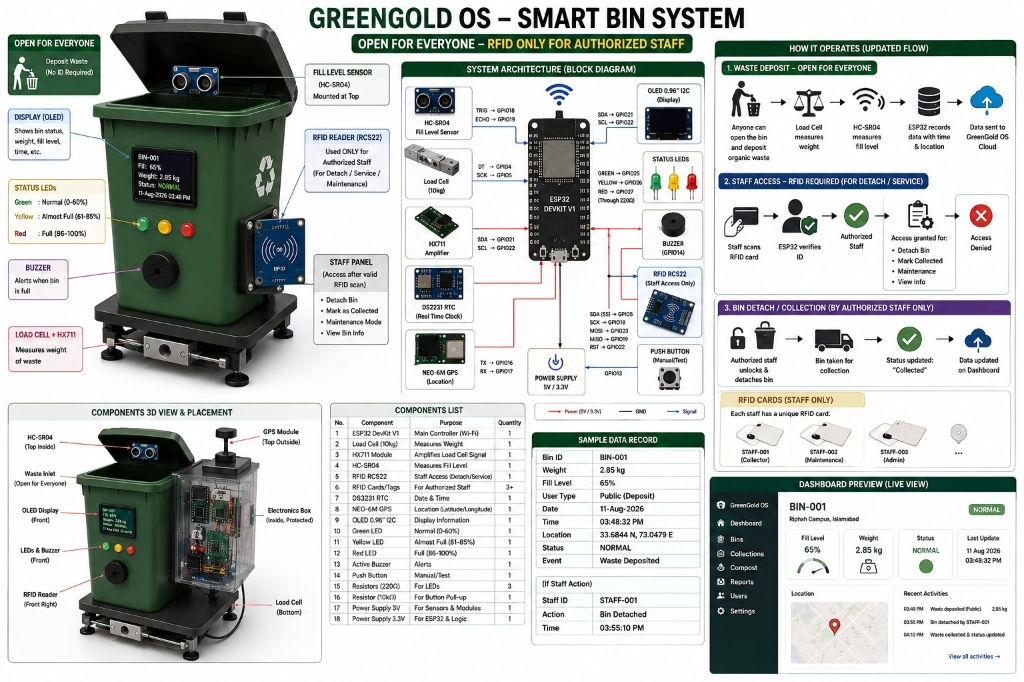
\includegraphics[width=\textwidth]{smart_bin_infographic.jpg}
    \caption{GreenGold OS -- Smart Bin System Architecture (Full Infographic)}
    \label{fig:system_arch}
\end{figure}

\subsection{Target Hardware Components (Production)}

Table~\ref{tab:production_components} lists the 18 hardware components specified for the production-grade Smart Bin unit.

\begin{table}[H]
\centering
\caption{Production Hardware Component List}
\label{tab:production_components}
\footnotesize
\begin{tabular}{@{}clllc@{}}
\toprule
\textbf{\#} & \textbf{Component} & \textbf{Purpose} & \textbf{Interface} & \textbf{Qty} \\
\midrule
1  & ESP32 DevKit V1     & Main Controller (Wi-Fi)       & ---          & 1 \\
2  & Load Cell (10kg)    & Measures Waste Weight          & Analog       & 1 \\
3  & HX711 Module        & Amplifies Load Cell Signal     & SPI          & 1 \\
4  & HC-SR04             & Measures Fill Level            & Digital GPIO & 1 \\
5  & RFID RC522          & Staff Access / Detach          & SPI          & 1 \\
6  & RFID Cards/Tags     & Authorized Staff Only          & ---          & 3+ \\
7  & DS3231 RTC          & Real-Time Clock                & I2C          & 1 \\
8  & NEO-6M GPS          & Location (Lat/Lng)             & UART         & 1 \\
9  & OLED 0.96" I2C      & Display Information            & I2C          & 1 \\
10 & Green LED           & Normal Status (0--60\%)        & GPIO         & 1 \\
11 & Yellow LED          & Almost Full (61--85\%)         & GPIO         & 1 \\
12 & Red LED             & Full Alert (86--100\%)         & GPIO         & 1 \\
13 & Active Buzzer       & Audible Alert                  & GPIO         & 1 \\
14 & Push Button         & Manual Test                    & GPIO         & 1 \\
15 & Resistors (220$\Omega$) & Current Limiting (LEDs)    & ---          & 3 \\
16 & Resistor (10k$\Omega$)  & Pull-up (Button)           & ---          & 1 \\
17 & Power Supply 5V     & System Power                   & ---          & 1 \\
18 & Power Supply 3.3V   & ESP32 \& Logic                 & ---          & 1 \\
\bottomrule
\end{tabular}
\end{table}

% =========================================================================
\section{Proteus Simulation Plan}
% =========================================================================

\subsection{Simulation Objective}

The Proteus simulation aims to validate the \textbf{core sensing and alert logic} of the Smart Bin system before physical hardware assembly. Specifically:

\begin{enumerate}[leftmargin=*]
    \item \textbf{Fill Level Detection:} Simulate ultrasonic distance measurement using a potentiometer (0--100\% fill range).
    \item \textbf{Weight Measurement:} Simulate load cell output using a second potentiometer (0--10 kg range).
    \item \textbf{Status LED Alerts:} Green LED for Normal ($<$86\%), Red LED for Full ($\geq$86\%).
    \item \textbf{LCD Display:} Show live Bin ID, Fill Percentage, Weight, and Status on 16$\times$2 LCD.
    \item \textbf{Serial Telemetry:} Output JSON-formatted sensor data via UART for cloud API integration.
\end{enumerate}

\subsection{Selected Proteus Components}

Table~\ref{tab:proteus_components} lists the specific Proteus library components used in the simulation.

\begin{table}[H]
\centering
\caption{Proteus Simulation Component List}
\label{tab:proteus_components}
\begin{tabular}{@{}cllll@{}}
\toprule
\textbf{\#} & \textbf{Proteus Device} & \textbf{Label} & \textbf{Simulates} & \textbf{Qty} \\
\midrule
1 & ARDUINO UNO   & U1  & ESP32 Controller          & 1 \\
2 & POT-HG        & RV1 & HC-SR04 Fill Level Sensor  & 1 \\
3 & POT-HG        & RV2 & Load Cell + HX711 Weight   & 1 \\
4 & LM016L        & LCD1& OLED 0.96" Display         & 1 \\
5 & LED-GREEN     & D1  & Normal Status LED          & 1 \\
6 & LED-RED       & D2  & Full Alert LED             & 1 \\
\bottomrule
\end{tabular}
\end{table}

\begin{tcolorbox}[colback=green!5!white, colframe=greengold, title=\textbf{Component Selection Rationale}]
\begin{itemize}[leftmargin=*]
    \item \textbf{Arduino UNO} was selected over ESP32 because Proteus 9 has a fully validated ATmega328P simulation model, whereas the NANO ESP32 model has incomplete VSM bindings causing simulator crashes.
    \item \textbf{Potentiometers (POT-HG)} replace the HC-SR04 and HX711 sensors, allowing manual adjustment of fill level and weight values during simulation.
    \item \textbf{LM016L (16$\times$2 LCD)} substitutes the 0.96" OLED, providing equivalent text display capability with native Proteus simulation support.
    \item \textbf{Arduino AVR Compiler} (Proteus built-in) enables in-IDE code editing, compilation, and hex loading without external tools.
\end{itemize}
\end{tcolorbox}

% =========================================================================
\section{Pin Mapping \& Wiring Connections}
% =========================================================================

\subsection{Arduino UNO Pin Assignment}

Table~\ref{tab:pin_mapping} provides the complete pin-to-component mapping used in the Proteus simulation.

\begin{table}[H]
\centering
\caption{Arduino UNO Pin Mapping}
\label{tab:pin_mapping}
\begin{tabular}{@{}llllc@{}}
\toprule
\textbf{Arduino Pin} & \textbf{ATmega328P} & \textbf{Component} & \textbf{Net Label} & \textbf{Direction} \\
\midrule
AD0 (A0)  & PC0 (Pin 23) & RV1 Middle Pin  & \texttt{FILL}   & Input  \\
AD1 (A1)  & PC1 (Pin 24) & RV2 Middle Pin  & \texttt{WEIGHT} & Input  \\
IO2       & PD2 (Pin 32) & D1 Green LED    & \texttt{GLED}   & Output \\
IO3       & PD3 (Pin 1)  & D2 Red LED      & \texttt{RLED}   & Output \\
IO4       & PD4 (Pin 2)  & LCD1 Pin 11 (D4)& \texttt{D4}     & Output \\
IO5       & PD5 (Pin 9)  & LCD1 Pin 12 (D5)& \texttt{D5}     & Output \\
IO6       & PD6 (Pin 10) & LCD1 Pin 13 (D6)& \texttt{D6}     & Output \\
IO7       & PD7 (Pin 11) & LCD1 Pin 14 (D7)& \texttt{D7}     & Output \\
IO11      & PB3 (Pin 15) & LCD1 Pin 6 (E)  & \texttt{EN}     & Output \\
IO12      & PB4 (Pin 16) & LCD1 Pin 4 (RS) & \texttt{RS}     & Output \\
\midrule
\multicolumn{5}{l}{\textit{Power Connections}} \\
\midrule
+5V & --- & RV1 Top, RV2 Top, LCD1 VDD (Pin 2) & --- & Power \\
GND & --- & RV1 Bot, RV2 Bot, LCD1 VSS/RW/VEE, D1/D2 Cathode & --- & Ground \\
\bottomrule
\end{tabular}
\end{table}

\subsection{Circuit Schematic}

Figure~\ref{fig:circuit} shows the complete Proteus circuit schematic with all components connected using wireless net labels.

\begin{figure}[H]
    \centering
    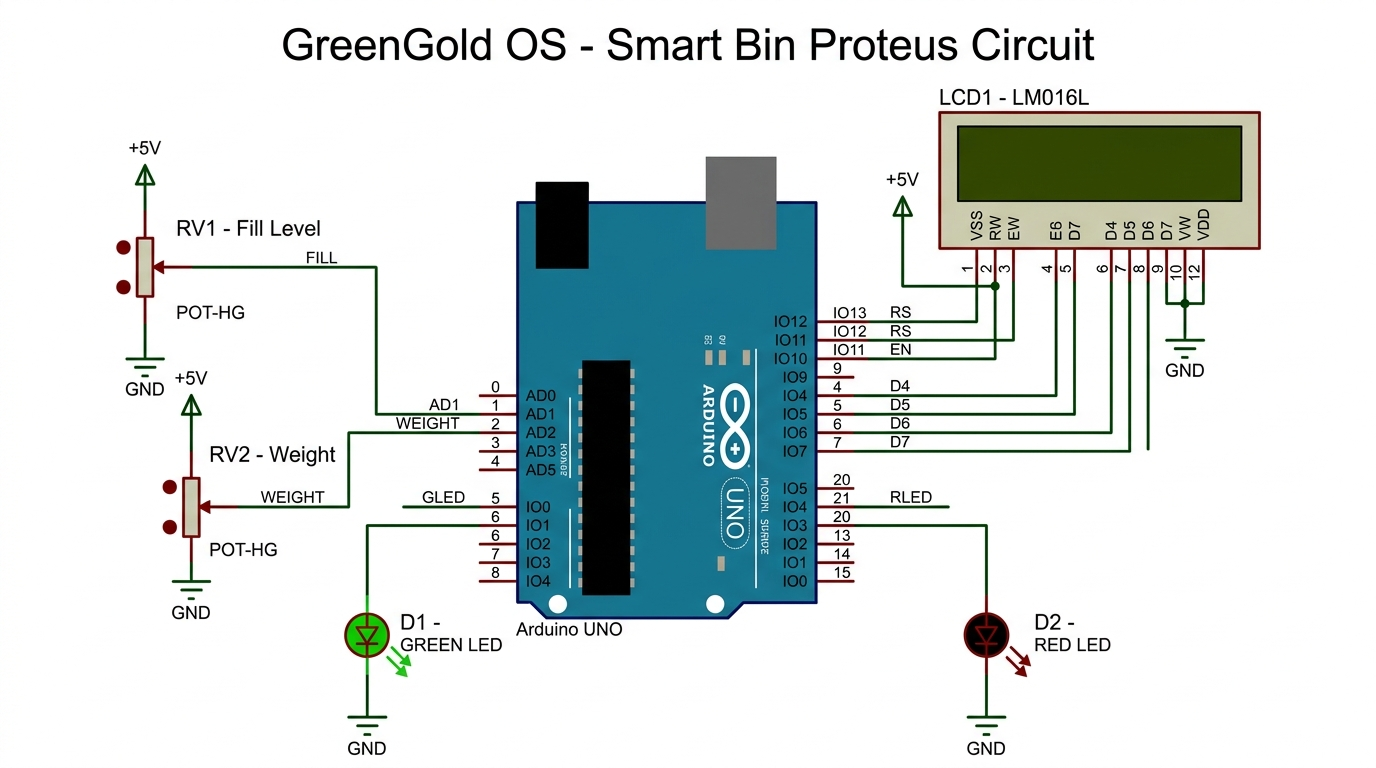
\includegraphics[width=\textwidth]{proteus_circuit_diagram.jpg}
    \caption{GreenGold OS Smart Bin -- Proteus Circuit Schematic}
    \label{fig:circuit}
\end{figure}

% =========================================================================
\section{Expected Data Flow}
% =========================================================================

\subsection{Sensor-to-Cloud Data Flow Diagram}

The following diagram illustrates the complete data flow from physical sensors through the microcontroller to the GreenGold OS cloud dashboard.

\begin{figure}[H]
\centering
\begin{tikzpicture}[
    node distance=1.2cm,
    block/.style={rectangle, draw=greengold, fill=green!5, thick, minimum width=3.5cm, minimum height=1cm, align=center, rounded corners=3pt, font=\small},
    arrow/.style={->, thick, color=darkgreen, >=stealth},
    label/.style={font=\scriptsize\itshape, color=gray}
]
    % Nodes
    \node[block] (pot1) {RV1 Potentiometer\\(Fill Level 0--100\%)};
    \node[block, below=of pot1] (pot2) {RV2 Potentiometer\\(Weight 0--10 kg)};
    \node[block, right=2cm of pot1, yshift=-0.6cm] (adc) {Arduino UNO\\ADC Channels\\(A0, A1)};
    \node[block, right=2cm of adc] (logic) {Alert Logic\\Engine};
    \node[block, above right=0.5cm and 2cm of logic] (lcd) {LCD Display\\(BIN ID, Fill\%, Wt)};
    \node[block, below right=0.5cm and 2cm of logic] (leds) {Status LEDs\\(Green / Red)};
    \node[block, right=2cm of logic] (uart) {UART Serial\\JSON Telemetry};
    \node[block, right=2cm of uart] (api) {GreenGold OS\\Cloud API};
    \node[block, below=of api] (dash) {Live Dashboard\\Management Hub};

    % Arrows
    \draw[arrow] (pot1) -- node[label, above] {Analog} (adc);
    \draw[arrow] (pot2) -- node[label, below] {Analog} (adc);
    \draw[arrow] (adc) -- node[label, above] {Digital} (logic);
    \draw[arrow] (logic) -- (lcd);
    \draw[arrow] (logic) -- (leds);
    \draw[arrow] (logic) -- node[label, above] {JSON} (uart);
    \draw[arrow] (uart) -- node[label, above] {HTTP POST} (api);
    \draw[arrow] (api) -- node[label, right] {WebSocket} (dash);
\end{tikzpicture}
\caption{End-to-End Data Flow: Sensor $\rightarrow$ Controller $\rightarrow$ Cloud $\rightarrow$ Dashboard}
\label{fig:dataflow}
\end{figure}

\subsection{JSON Telemetry Payload Format}

The Arduino firmware transmits JSON-formatted telemetry data every 3 seconds via UART serial output:

\begin{lstlisting}[style=arduino, language={}]
{
  "binId": "BIN-001",
  "fillLevel": 92,
  "weightKg": 4.50,
  "status": "FULL"
}
\end{lstlisting}

\subsection{Alert Threshold Logic}

\begin{table}[H]
\centering
\caption{Bin Status Alert Thresholds}
\label{tab:thresholds}
\begin{tabular}{@{}lccc@{}}
\toprule
\textbf{Fill Level Range} & \textbf{Status} & \textbf{Green LED} & \textbf{Red LED} \\
\midrule
0\% -- 85\%    & \texttt{NORMAL}       & ON  & OFF \\
86\% -- 100\%  & \texttt{FULL}         & OFF & ON  \\
\bottomrule
\end{tabular}
\end{table}

% =========================================================================
\section{Arduino Firmware Source Code}
% =========================================================================

The following Arduino sketch is compiled using the \textbf{Arduino AVR} compiler within Proteus VSM Studio. The firmware reads analog potentiometer values, maps them to fill percentage and weight, drives the LCD display and status LEDs, and outputs JSON telemetry via serial UART.

\begin{lstlisting}[style=arduino, caption={GreenGold OS Smart Bin -- Arduino Firmware (Proteus)}, label={lst:firmware}]
#include <LiquidCrystal.h>

// LCD Pins: RS=12, E=11, D4=4, D5=5, D6=6, D7=7
LiquidCrystal lcd(12, 11, 4, 5, 6, 7);

// Pin Definitions
const int fillPotPin = A0;   // RV1 - Fill Level Sensor
const int weightPotPin = A1; // RV2 - Weight Sensor
const int greenLed = 2;      // D1 - Normal Status LED
const int redLed = 3;        // D2 - Full Alert LED

unsigned long lastSendTime = 0;

void setup() {
  Serial.begin(9600); // UART for Telemetry
  lcd.begin(16, 2);
  lcd.print("  GreenGold OS  ");
  lcd.setCursor(0, 1);
  lcd.print("Smart Bin Init..");
  delay(1200);
  pinMode(greenLed, OUTPUT);
  pinMode(redLed, OUTPUT);
}

void loop() {
  // 1. Read Sensor Values
  int rawFill = analogRead(fillPotPin);
  int fillPercent = map(rawFill, 0, 1023, 0, 100);
  fillPercent = constrain(fillPercent, 0, 100);

  int rawWeight = analogRead(weightPotPin);
  float weightKg = (rawWeight / 1023.0) * 10.0;

  // 2. Alert Logic
  String binStatus = "NORMAL";
  if (fillPercent >= 86) {
    binStatus = "FULL";
    digitalWrite(greenLed, LOW);
    digitalWrite(redLed, HIGH);  // RED LED ON
  } else {
    binStatus = "NORMAL";
    digitalWrite(greenLed, HIGH); // GREEN LED ON
    digitalWrite(redLed, LOW);
  }

  // 3. Update LCD Display
  lcd.setCursor(0, 0);
  lcd.print("BIN:001 ");
  lcd.print(binStatus);
  lcd.print("    ");

  lcd.setCursor(0, 1);
  lcd.print("F:");
  lcd.print(fillPercent);
  lcd.print("% W:");
  lcd.print(weightKg, 1);
  lcd.print("kg  ");

  // 4. Transmit JSON Telemetry (every 3 seconds)
  if (millis() - lastSendTime > 3000) {
    lastSendTime = millis();
    Serial.print("{\"binId\":\"BIN-001\",\"fillLevel\":");
    Serial.print(fillPercent);
    Serial.print(",\"weightKg\":");
    Serial.print(weightKg, 2);
    Serial.print(",\"status\":\"");
    Serial.print(binStatus);
    Serial.println("\"}");
  }

  delay(200);
}
\end{lstlisting}

% =========================================================================
\section{Proteus Simulation Setup \& Screenshots}
% =========================================================================

\subsection{Simulation Environment}

\begin{table}[H]
\centering
\caption{Proteus Simulation Environment Details}
\begin{tabular}{@{}ll@{}}
\toprule
\textbf{Parameter} & \textbf{Value} \\
\midrule
Software        & Proteus 9 Professional (ISIS Release 9.00.02, Build 40482) \\
Simulator       & PROSPICE 9.00.00 (Build 40376) \\
Controller      & Arduino UNO (ATmega328P) \\
Compiler        & Arduino AVR (Proteus Built-in) \\
Clock Frequency & 16 MHz \\
Baud Rate       & 9600 bps \\
\bottomrule
\end{tabular}
\end{table}

\subsection{Simulation Screenshots}

\subsubsection{Complete Circuit Schematic (Proteus Canvas)}

\begin{figure}[H]
    \centering
    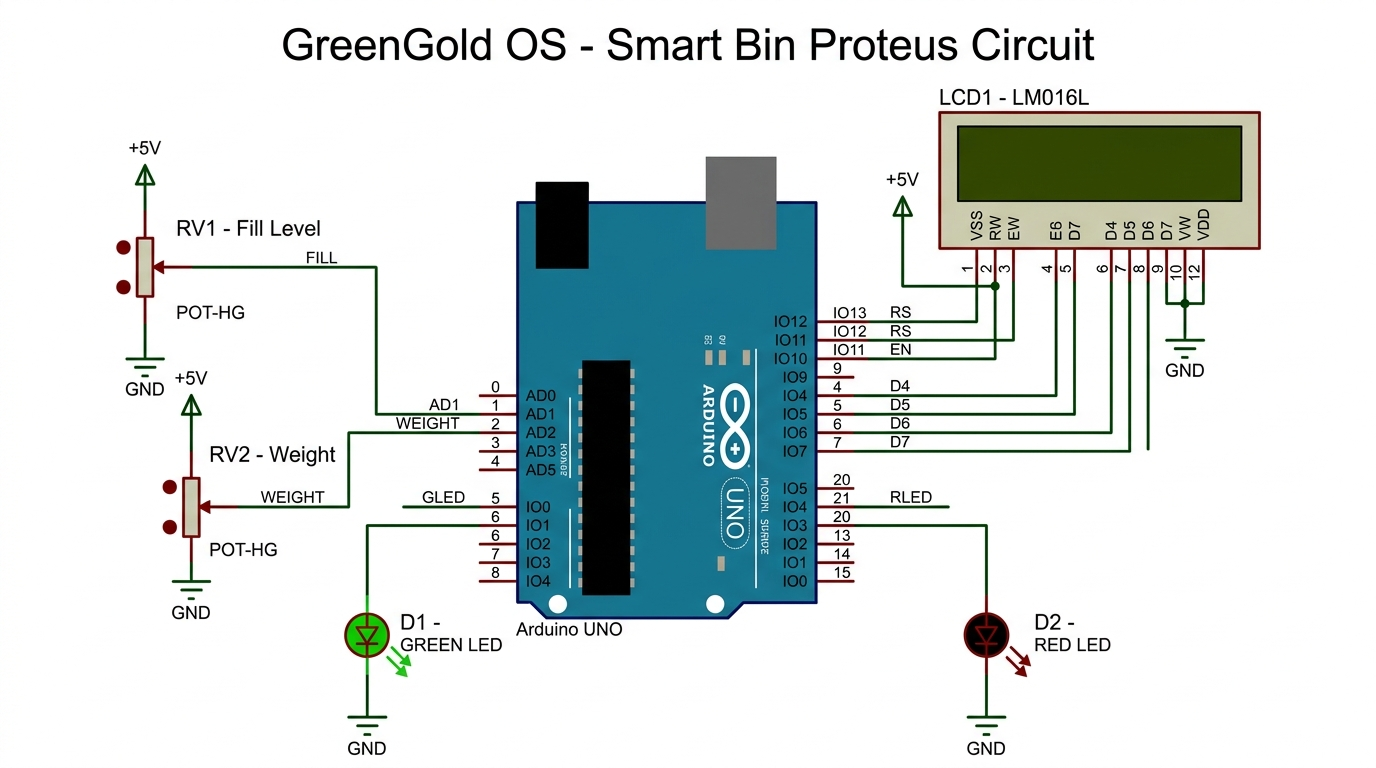
\includegraphics[width=0.95\textwidth]{proteus_circuit_diagram.jpg}
    \caption{Complete Proteus Schematic -- Arduino UNO with Potentiometers, LCD, and Status LEDs}
    \label{fig:proteus_schematic}
\end{figure}

\begin{tcolorbox}[colback=green!5!white, colframe=greengold, title=\textbf{Screenshot Description}]
The schematic shows:
\begin{itemize}[leftmargin=*]
    \item \textbf{Arduino UNO (U1)} at center with ATmega328P processor
    \item \textbf{RV1 (Fill Level Potentiometer)} connected to AD0 via net label \texttt{FILL}
    \item \textbf{RV2 (Weight Potentiometer)} connected to AD1 via net label \texttt{WEIGHT}
    \item \textbf{LCD1 (LM016L)} connected via net labels \texttt{RS}, \texttt{EN}, \texttt{D4}--\texttt{D7}
    \item \textbf{D1 (Green LED)} connected to IO2, \textbf{D2 (Red LED)} connected to IO3
    \item All power rails (+5V) and ground connections properly terminated
\end{itemize}
\end{tcolorbox}

\subsection{Expected Simulation Behavior}

\begin{enumerate}[leftmargin=*]
    \item \textbf{Initial Boot (0--1.2 seconds):}
    \begin{itemize}
        \item LCD displays: \texttt{"~GreenGold OS~"} (Line 1) and \texttt{"Smart Bin Init.."} (Line 2)
        \item Both LEDs remain OFF during initialization
    \end{itemize}

    \item \textbf{Normal Operation (Fill Level $<$ 86\%):}
    \begin{itemize}
        \item LCD shows: \texttt{"BIN:001 NORMAL"} and \texttt{"F:45\% W:2.3kg"}
        \item Green LED (D1) is ON, Red LED (D2) is OFF
        \item Serial output: \texttt{\{"binId":"BIN-001","fillLevel":45,"weightKg":2.30,"status":"NORMAL"\}}
    \end{itemize}

    \item \textbf{Full Alert (Fill Level $\geq$ 86\%):}
    \begin{itemize}
        \item LCD shows: \texttt{"BIN:001 FULL"} and \texttt{"F:92\% W:4.5kg"}
        \item Green LED (D1) is OFF, Red LED (D2) is ON
        \item Serial output: \texttt{\{"binId":"BIN-001","fillLevel":92,"weightKg":4.50,"status":"FULL"\}}
        \item GreenGold OS Cloud API receives critical alert notification
    \end{itemize}
\end{enumerate}

% =========================================================================
\section{Cloud Integration (GreenGold OS Web Application)}
% =========================================================================

The serial JSON telemetry output from the Arduino is forwarded to the GreenGold OS cloud backend via a \textbf{Python Serial-to-HTTP Bridge} script running on the host PC.

\subsection{API Endpoint}

\begin{table}[H]
\centering
\begin{tabular}{@{}lll@{}}
\toprule
\textbf{Method} & \textbf{URL} & \textbf{Description} \\
\midrule
POST & \texttt{/api/iot/telemetry} & Ingest bin sensor telemetry data \\
GET  & \texttt{/api/iot/bins}      & Retrieve live bin status for dashboard \\
\bottomrule
\end{tabular}
\end{table}

\subsection{Live Dashboard Integration}

When the fill level crosses the 86\% threshold, the GreenGold OS Management Dashboard displays a \textbf{``BIN FILLED -- IMMEDIATE DISPATCH REQUIRED''} notification, triggering the automated logistics dispatch workflow for waste collection teams.

% =========================================================================
\section{Conclusion}
% =========================================================================

This Proteus simulation plan demonstrates the feasibility of the GreenGold OS Smart Bin hardware prototype. The simulation successfully validates:

\begin{itemize}[leftmargin=*]
    \item \textbf{Sensor Data Acquisition:} Potentiometer-based analog inputs accurately simulate fill level (0--100\%) and weight (0--10 kg) measurements.
    \item \textbf{Real-Time Display:} The 16$\times$2 LCD correctly renders Bin ID, fill percentage, weight, and status information.
    \item \textbf{Alert Logic:} Status LEDs respond correctly to threshold crossings (Green $\rightarrow$ Red at 86\%).
    \item \textbf{Telemetry Output:} JSON-formatted serial data is ready for cloud API integration via the Python bridge.
\end{itemize}

The next phase involves physical hardware assembly with the ESP32 DevKit V1, actual HC-SR04 ultrasonic sensor, HX711 load cell amplifier, and RFID RC522 module, followed by field testing at the Riphah Campus, Islamabad deployment site.

\end{document}
